\section{Influence of Double Gene Gain Events}\label{app:double-p-value}
The influence of double gene gain events on low gene-count simulations with 10 samples and$\theta = 100, \rho = 0.1$.
The $\chi^2$-like values for simulations with less than 20000 genes show a significant deviation from the reference.

\begin{table}[H]
    \begin{tabular}{l|l|c}
        Number of sites & P Value  & Significant \\
        \hline
        1000            & 2.21e-05 & x           \\
        2000            & 8.16e-21 & x           \\
        5000            & 3.40e-09 & x           \\
        10000           & 8.59e-05 & x           \\
        20000           & 0.13     &             \\
        50000           & 0.31     &             \\
        100000          & 0.78     &             \\
        200000          & 0.80     &             \\
        500000          & 0.12     &
    \end{tabular}
    \caption{Effect of double gene-gains on the log-transformed $\chi^2$-like values for low number of sites simulations.}
\end{table}
\newpage
\section{Neutrality Test Robustness}
\begin{table}[h]
    \centering
    \begin{tabular}{r|llll}
        Parameter & start & stop   & step    & default \\
        \hline
        $\theta$  & 0     & 5000   & 10      & 1500    \\
        $\rho$    & 0.1   & 5      & 0.1     & 1       \\
        $\kappa$  & 0     & 4      & 0.1     & 0       \\
        $\gamma$  & 0     & 0.0005 & 0.00001 & 0
    \end{tabular}
    \caption{Neutrality test robustness parameters.}
    \label{app:robust-param}
\end{table}

\begin{figure}[H]
    \centering
    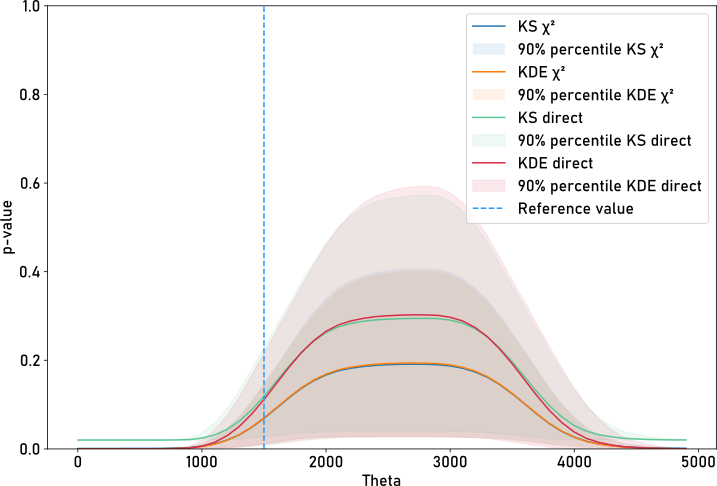
\includegraphics[width=0.49\textwidth]{figures/neutrality_test/gc_2_theta.pdf}
    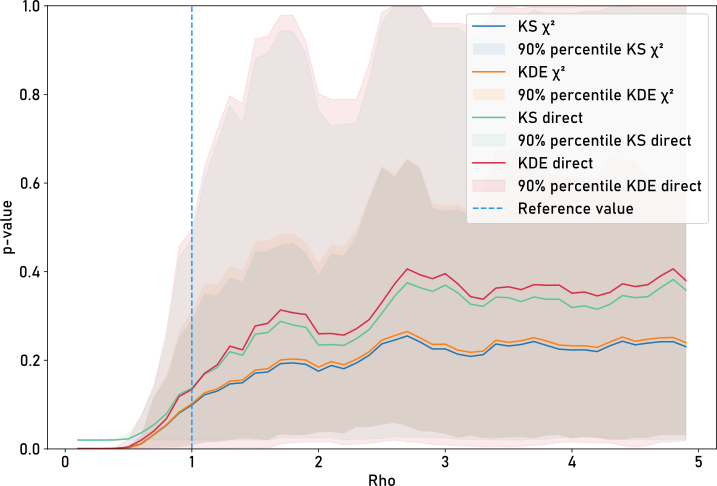
\includegraphics[width=0.49\textwidth]{figures/neutrality_test/gc_2_rho.pdf}
    \caption[Robustness of the neutrality test for $\kappa = 2$ as reference.]{Robustness of the neutrality test for different $\theta$ (left), $\rho$ (right) values
        with $\kappa = 2$ as reference.}
    \label{app:robust_gc}
\end{figure}
\newpage
\section{Runtime}\label{app:runtime}
The first differences of the recorded runtime of \mintinline{python}{gene_model} for different parameters and the absolute runtime for different $\theta / \rho$ ratios are presented here.

\begin{figure}[H]
    \centering
    \includegraphics[width=0.6\textwidth]{figures/runtime/theta_rho_heat.pdf}
    \caption[Runtime of $\theta / \rho$ ratios.]{Runtime of \mintinline{python}{gene_model} for different $\theta / \rho$ ratios for 10 samples and $\kappa = \gamma = 0$.}
    \label{app:theta-rho-heatmap}
\end{figure}
\begin{figure}[H]
    \begin{flushright}
        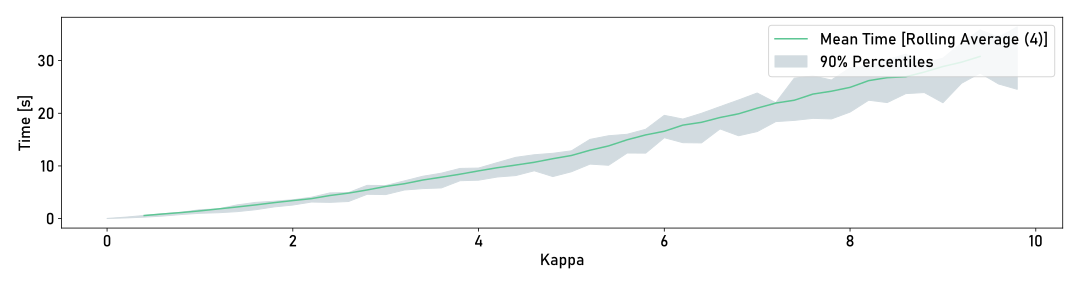
\includegraphics[width=0.988\textwidth]{figures/runtime/gene_conversion_rate_large.pdf}
    \end{flushright}
    \centering
    \caption[Runtime without HGT.]{Runtime of \mintinline{python}{gene_model} for different $\kappa$ rates for simulations without HGT.}
    \label{app:runtime-ext}
\end{figure}

\begin{figure}[H]
    \begin{flushright}
        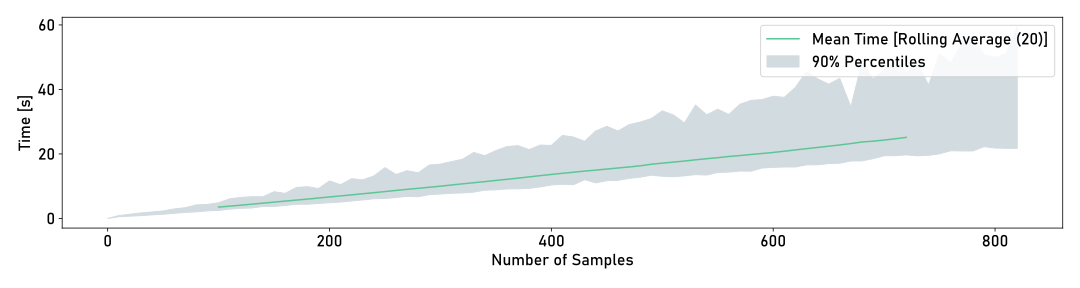
\includegraphics[width=0.995\textwidth]{figures/runtime/hgt_num_samples.pdf}\\
        \includegraphics[width=\textwidth]{figures/runtime/hgt_num_sites.pdf}\\
        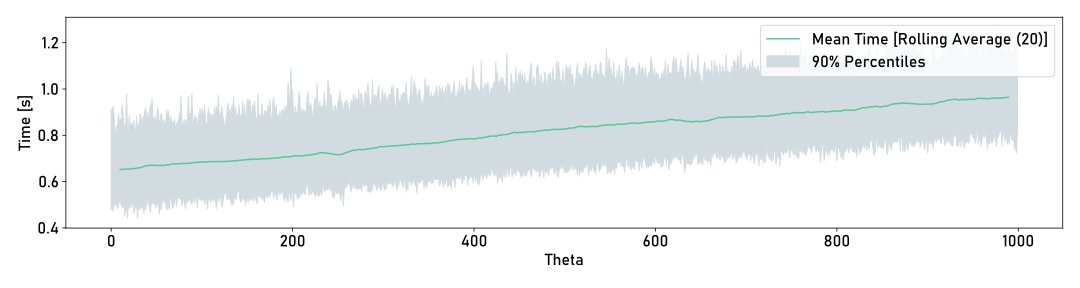
\includegraphics[width=\textwidth]{figures/runtime/hgt_theta.pdf}\\
        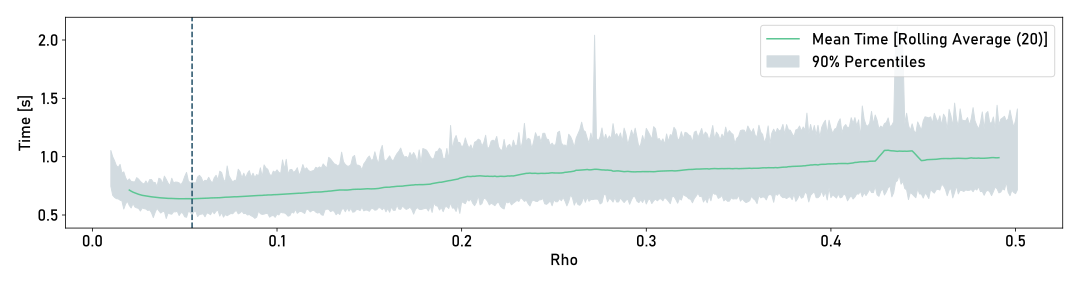
\includegraphics[width=\textwidth]{figures/runtime/hgt_rho.pdf}\\
        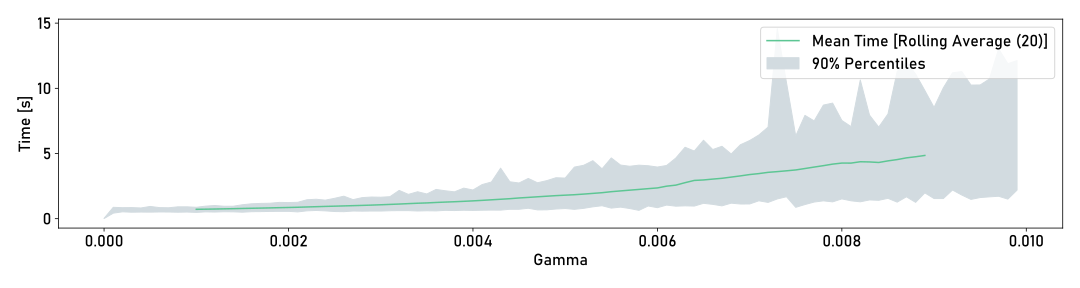
\includegraphics[width=0.995\textwidth]{figures/runtime/hgt_hgt_rate.pdf}
    \end{flushright}
    \centering
    \caption[Runtime with HGT.]{Runtime of \mintinline{python}{gene_model} for different number of samples, number of sites, $\theta$, $\rho$ and $\gamma$ rates
        for simulations with HGT.}
    \label{app:runtime-hgt}
\end{figure}
\begin{figure}[H]
    \begin{flushright}
        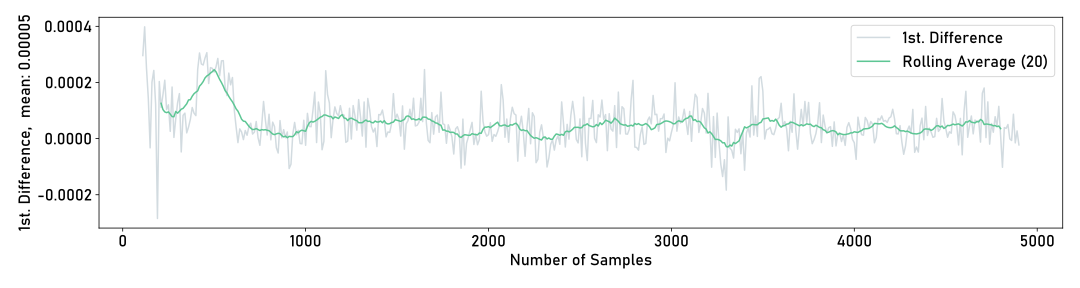
\includegraphics[width=\textwidth]{figures/runtime/num_samples_diff.pdf}\\
        \includegraphics[width=\textwidth]{figures/runtime/num_sites_diff.pdf}\\
        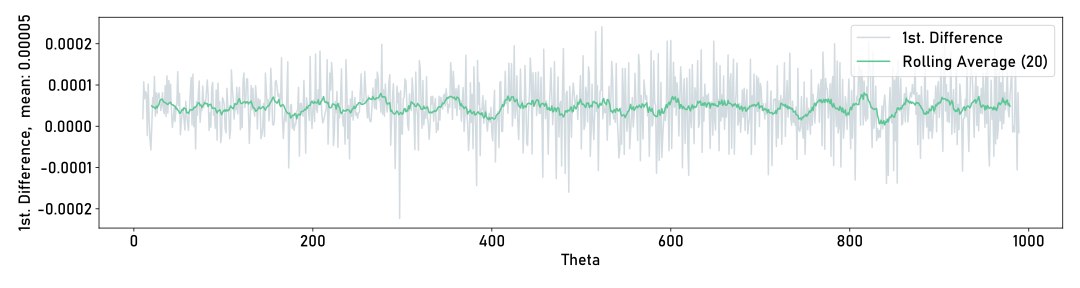
\includegraphics[width=\textwidth]{figures/runtime/theta_diff.pdf}\\
        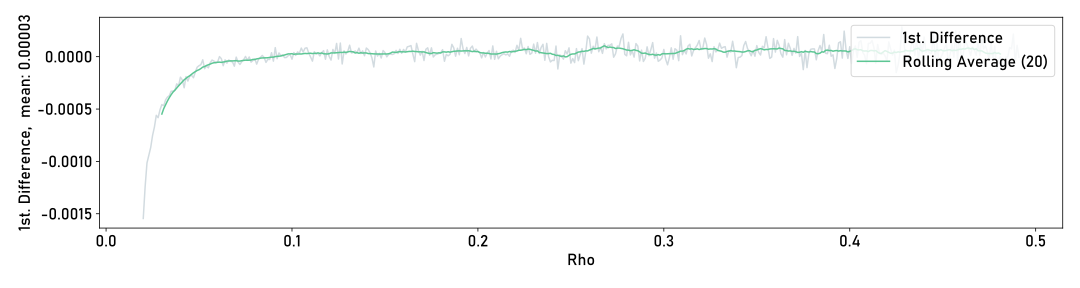
\includegraphics[width=\textwidth]{figures/runtime/rho_diff.pdf}\\
        \includegraphics[width=0.975\textwidth]{figures/runtime/gene_conversion_rate_large_diff.pdf}
    \end{flushright}
    \centering
    \caption[First difference of runtime without HGT.]{First difference of runtime of \mintinline{python}{gene_model} for different number of samples, number of sites, $\theta$, $\rho$ and $\kappa$ rates
        for simulations without HGT.}
    \label{app:diff-runtime}
\end{figure}

\begin{figure}[H]
    \begin{flushright}
        \includegraphics[width=0.983\textwidth]{figures/runtime/hgt_num_samples_diff.pdf}\\
        \includegraphics[width=0.992\textwidth]{figures/runtime/hgt_num_sites_diff.pdf}\\
        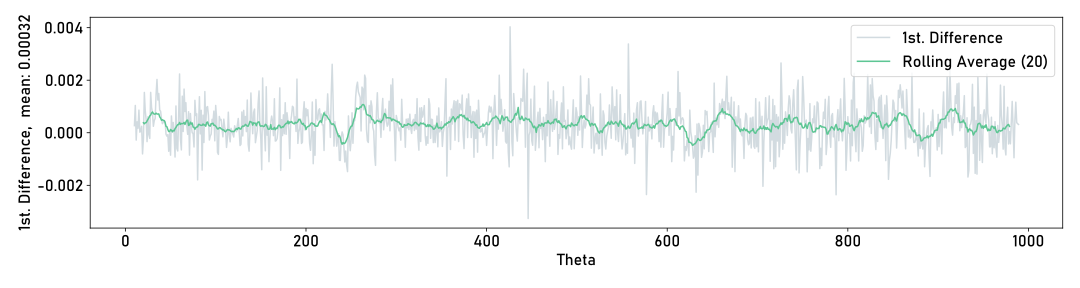
\includegraphics[width=\textwidth]{figures/runtime/hgt_theta_diff.pdf}\\
        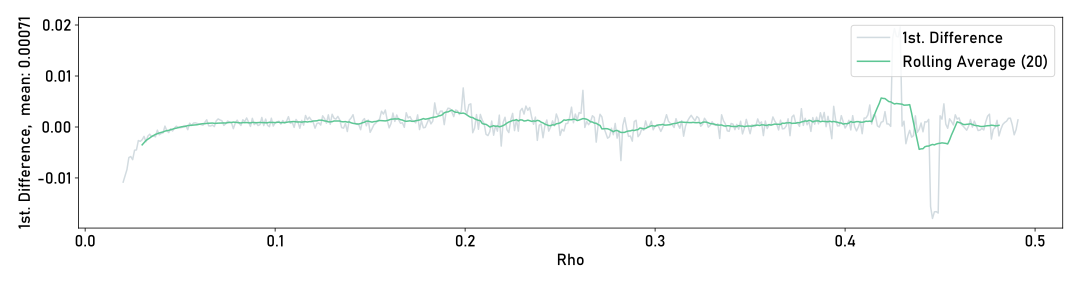
\includegraphics[width=0.988\textwidth]{figures/runtime/hgt_rho_diff.pdf}\\
        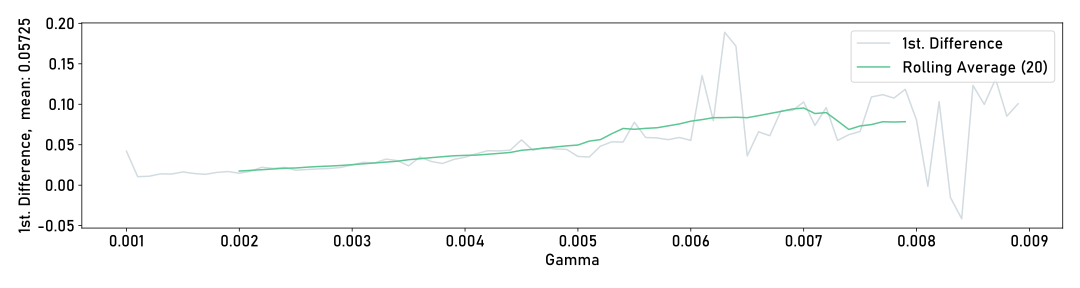
\includegraphics[width=0.988\textwidth]{figures/runtime/hgt_hgt_rate_diff.pdf}
    \end{flushright}
    \centering
    \caption[First difference of runtime with HGT.]{First difference of runtime of \mintinline{python}{gene_model} for different number of samples, number of sites, $\theta$, $\rho$ and $\gamma$ rates
        for simulations with HGT.}
    \label{app:diff-runtime-hgt}
\end{figure}
\section{Trees for parameter estimation}
\begin{figure}[H]
    \begin{flushleft}
        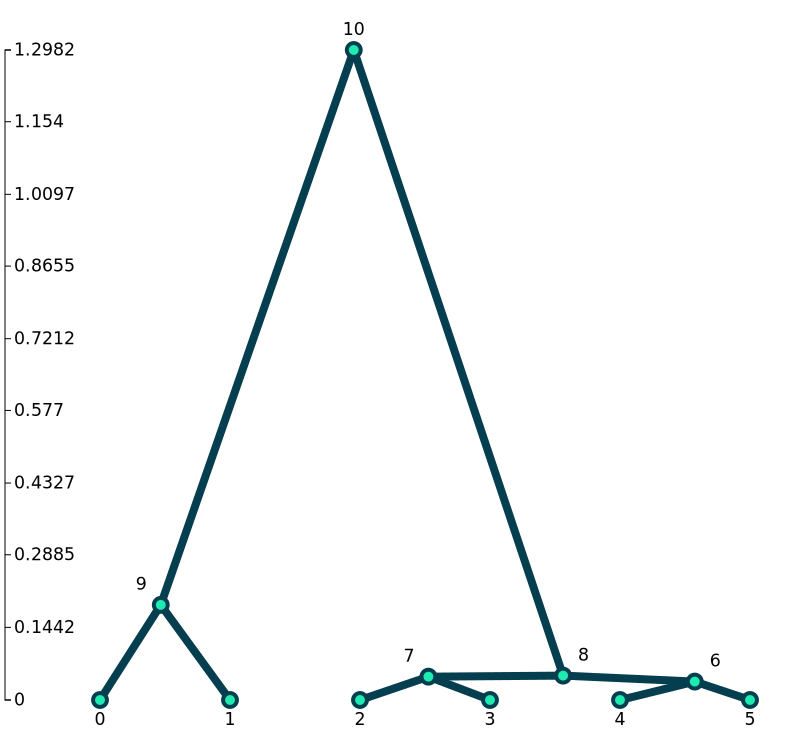
\includegraphics[width=0.49\textwidth]{figures/panX_trees/803.pdf}
        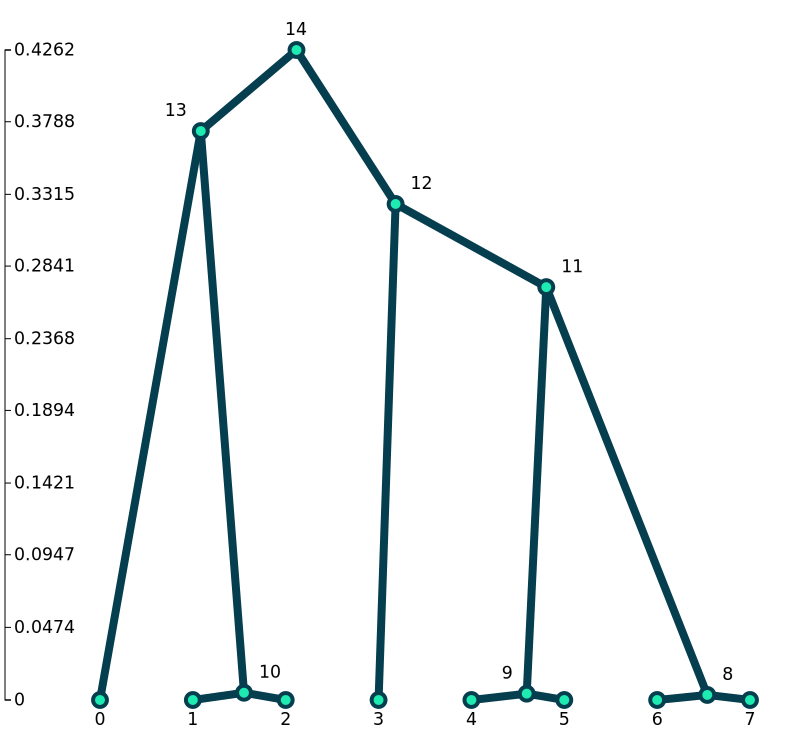
\includegraphics[width=0.49\textwidth]{figures/panX_trees/985002.pdf}\\
        \includegraphics[width=0.49\textwidth]{figures/panX_trees/1492.pdf}\\
        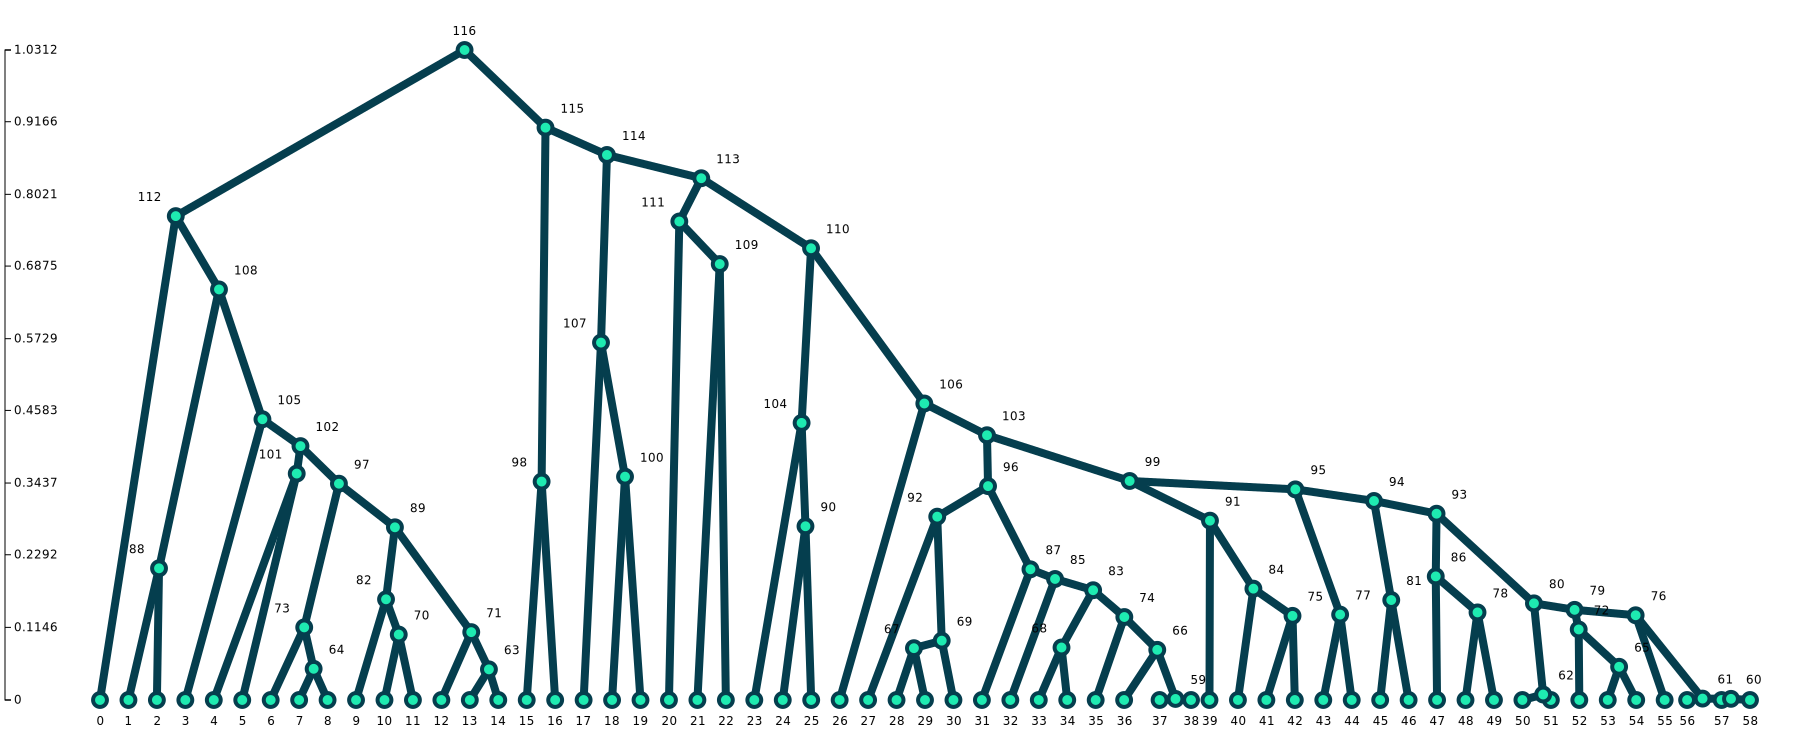
\includegraphics[width=\textwidth]{figures/panX_trees/9.pdf}
    \end{flushleft}
    \centering
    \caption[Trees for parameter estimation.]{Phylogenetic trees inferred by \textit{PanX} and used for parameter estimation.
        From top to bottom: Bartonella quintana, Staphylococcus argenteus, Clostridium butyricum and Buchnera aphidicola.}
    \label{app:panX-trees}
\end{figure}

\section{Software and Package Versions}
\begin{table}[H]
    %\begin{adjustbox}{width=\textwidth}
    \begin{tabular}{l|l|l}
        Name                 & Version & Reference                                                                                    \\
        \hline
        bintrees             & 2.2.0   & \href{https://pypi.org/project/bintrees/}{pypi.org/project/bintrees}                         \\
        matplotlib           & 3.8.0   & \href{https://matplotlib.org/}{matplotlib.org}                                               \\
        msprime              & 1.3.1   & \href{https://tskit.dev/software/msprime.html}{tskit.dev/software/msprime.html}              \\
        numpy                & 1.26.4  & \href{https://numpy.org/}{numpy.org/}                                                        \\
        pandas               & 2.2.0   & \href{https://pandas.pydata.org/}{pandas.pydata.org}                                         \\
        python               & 3.12.1  & \href{https://www.python.org/}{python.org}                                                   \\
        scipy                & 1.12.0  & \href{https://scipy.org/}{scipy.org}                                                         \\
        seaborn              & 0.12.2  & \href{https://seaborn.pydata.org/}{seaborn.pydata.org}                                       \\
        statsmodels          & 0.14.1  & \href{https://www.statsmodels.org/stable/index.html}{statsmodels.org/stable}                 \\
        tskit                & 0.5.6   & \href{https://tskit.dev/software/tskit.html}{tskit.dev/software/tskit.html}                  \\
        tskit-arg-visualizer & 0.0.1   & \href{https://pypi.org/project/tskit-arg-visualizer/}{pypi.org/project/tskit-arg-visualizer}
    \end{tabular}
    %\end{adjustbox}
    \label{app:package-versions}
\end{table}
An installable conda environment is available on GitHub:\\
\href{https://github.com/not-a-feature/pangenome-gene-transfer-simulation/blob/main/conda_env.yml}{pangenome-gene-transfer-simulation/blob/main/conda\_env.yml}.

\section{Sustainability}
Most of the simulations were run on an Intel \textsuperscript{\textregistered} Core \texttrademark ~i5-13500 processor with a peak power consumption of 154W.
Taking into account additional overheads for cooling, idle GPU and other components, the estimated total power consumption is 200W.
The remaining simulations were run on an AMD Ryzen \texttrademark ~Threadripper \texttrademark ~3970X 32-core processor with a peak power consumption of 280W.
This would give an approximate total power consumption of 350W.
Total test and simulation durations were estimated at 350 and 50 hours respectively.

The resulting energy consumption was 87.5 kWh, supplied by a 100\% renewable energy supplier.